% CircusTent Section

%\begin{figure*}[!t]
%\centering
%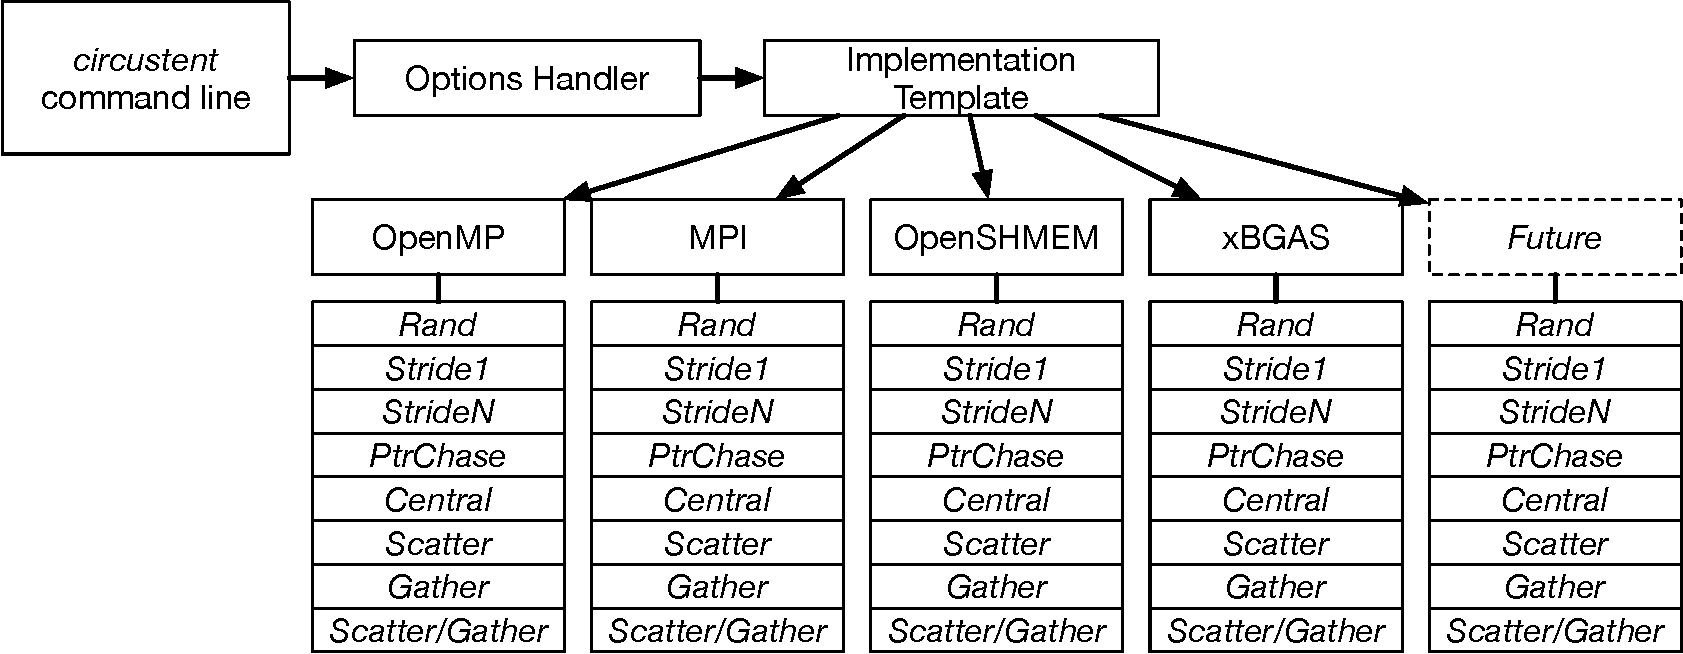
\includegraphics[width=5in]{figures/arch.pdf}
%\caption{CircusTent Architecture}
%\label{fig:ct_arch}
%\end{figure*}

\subsection{Benchmark Overview}
\label{subsec:benchmark_overview}

The CircusTent benchmark infrastructure is designed to provide users and system architects the ability to derive normalized, quantitative performance data for atomic memory operations on parallel systems.  For this, we defined the following driving requirements.  

\subsubsection*{Derivation of Normalized Results}

One of the primary difficulties in designing future scalable systems is the ability to derive and utilize quantifiable data to assist in the process of evaluating architectural trade offs.
While application benchmark data is of paramount importance, it is often difficult to synthesize performance characteristics across applications or application kernels.
As a result, the CircusTent benchmark derives a normalized, quantifiable performance value regardless of the size and implementation of the target system.  

\subsubsection*{Programming Model Support}

One of the unique characteristics of the CircusTent infrastructure is its ability to support a multitude of programming models for shared and distributed memory utilizing heterogeneous system architectures.
Unlike previous memory benchmarks that were implemented using a single programming model, CircusTent seeks to exploit the intersection of the system architecture and programming model.
Disparate programming models present atomic memory operations using a variety of methods that include compiler intrinsics, programming model directives, and explicit function calls.
Therefore, CircusTent permits architects to utilize the benchmark with the application programming model most relevant to their constituent users. 

\subsubsection*{System-Specific Optimizations}

In addition to supporting a myriad of programming model backends, the CircusTent infrastructure also has the ability to support system-specific optimizations.
As each programming model implementation is supported via a base implementation template, users have the ability to prescriptively utilize system-specific optimizations such as inline assembly language or compiler intrinsics to induce system-specific behavior.

\subsubsection*{Pathological Kernels}

Finally, in order to mimic a wide array of application memory access patterns, CircusTent is designed to support eight pathological kernels that replicate common memory access patterns of interest.
The patterns include unit stride, non unit stride, irregular, or entirely random accesses to memory locations using a variety of loop constructs.
Further, each pathological kernel can be implemented using various different styles of atomic memory operations.
We currently implement CircusTent backends using atomic \textit{Add} and \textit{Compare-and-Swap}.    

As we see in Figure~\ref{fig:ct_arch}, the CircusTent infrastructure is constructed using a C++ inheritance model whereby operations such as command line parsing and benchmark option handling are common across all supported programming models.
The implementation template is a C++ base class that is utilized to encapsulate each individual programming model implementation.
Operations such as memory allocation, deallocation, and programming model initialization are provided by base-level member routines that are overridden by each respective programming model.
In this manner, each programming model implementation has the ability to utilize it's respective initialization and allocation routines.

In addition to the aforementioned initialization and allocation routine functions, each programming is also required to implement individual versions of each benchmark algorithm (Section~\ref{subsec:algorithms}).
For each algorithm defined, the implementation can be optimized using the respective programming model constructs in order to induce optimal performance.    

\subsection{Programming Models}
\label{subsec:programming_models}

The current set of programming models supported by CircusTent includes OpenMP, MPI, OpenSHMEM, and xBGAS~\cite{leidel2018xbgas}.
As mentioned above, each respective implementation contains a unique set of initialization, memory allocation, and execution functions.
The initialization functions perform any necessary device discovery, library initialization, and rudimentary setup as required for each programming model.
Similarly, the memory allocation routines are utilized by each programming model to allocate and initialize two data structures.
The \texttt{VAL} data structure is a linear array that that may span multiple nodes and contains target data.
The \textit{IDX} data structure is also a linear array that may span multiples nodes and contains indices within the scope of the \texttt{VAL} data structure.
Currently, all the backend implementations utilize unsigned 64-bit integers (\texttt{uint64\_t}) for each data and index value.  
Notably, the initialization and allocation time is not included in the algorithmic runtime reported by the top-level driver functions.
Finally, each of the respective models contains an optimized implementation of each kernel that utilizes both target atomic memory operation types, (\textit{atomic add} and \textit{compare and swap}).

\subsubsection{OpenMP}
\label{subsubsec:openmp}

The first programming model utilized to implement a CircusTent backend is OpenMP.  
The OpenMP backend is rather simple and does not include a large number of CPU or memory-specific optimizations.
As OpenMP is utilized in only physically shared memory environments, this backend employs standard \texttt{malloc} routines for the \texttt{VAL} and \texttt{IDX} memory management.
Further, as we sought to make the OpenMP backend as portable as possible, it does not utilize any explicit NUMA optimizations. 
For each of the target kernels, we utilize the OpenMP \texttt{for} loop construct to parallelize the algorithms across multiple PEs.
The default scheduling paradigm, as defined by the OpenMP runtime, is also utilized.
For each atomic operation, we exploit the GNU atomic builtins using the \texttt{\_\_ATOMIC\_RELAXED} argument such that architectures with weak memory ordering may have multiple requests in flight.  

\subsubsection{MPI}
\label{subsubsec:mpi}

The second programming model utilized to implement a CircusTent backend is MPI.  
Specifically, we utilize the MPI-3 specification~\cite{mpi-3.0}~\cite{10.1007/978-3-642-33518-1_1} to implement this distributed memory backend.
The MPI backend is constructed using MPI-3 \textit{window} constructs for dynamic, one-sided RMA operations.
Each of the \texttt{VAL} and \texttt{IDX} constructs are locally allocated and mapped into a dynamic window.
Within the kernel implementations of each algorithm, we utilize one sided operations, \texttt{MPI\_Get} and \texttt{MPI\_Put}, to fetch normal index values.
Similarly, the \texttt{MPI\_Compare\_and\_swap} and \texttt{MPI\_Fetch\_and\_op} MPI-3 atomic operation function calls are utilized for realization of the actual atomics.
Depending upon the MPI library utilized at compile time, each of the aforementioned MPI atomic operations may be implemented utilizing combinations of OS system calls, microarchitectural atomic 
operations, and remote direct memory access (RDMA) operations on the interconnect.  

\subsubsection{OpenSHMEM}
\label{subsubsec:openshmem}

The next programming model utilized to implement a CircusTent backend is OpenSHMEM~\cite{openshmemspec}~\cite{Poole2011}.
OpenSHMEM consists of a runtime infrastructure and set of common function interfaces that provide distributed memory systems a shared memory view via a symmetric heap managed by the runtime.  
Similar to other parallel programming models such as MPI, OpenSHMEM provides native interfaces for atomics, one-sided communication, as well as native memory allocation routines.
For CircusTent, we utilize the standard set of OpenSHMEM memory management routines (\texttt{shmem\_malloc}) in order to allocate the \texttt{VAL} and \texttt{IDX} constructs in the symmetric heap.
Similar to the MPI-3 implementation, we utilize native OpenSHMEM one-sided operations, \texttt{shmem\_long\_get} and \texttt{shmem\_long\_put}, to fetch normal index values.
We utilize the native OpenSHMEM atomic function interfaces, \texttt{shmem\_long\_fadd} and \texttt{shmem\_long\_cswap}, for atomic add and compare-and-swap, respectively.  

\subsubsection{xBGAS}
\label{subsubsec:xbgas}
The final programming model currently utilized to implement a CircusTent backend is the xBGAS runtime infrastructure~\cite{leidel2018xbgas}~\cite{xbgasspec}.
xBGAS is a project to construct a microarchitectural extension to the RISC-V instruction set in order to provide instruction-level shared memory access across distributed memory systems.
The xBGAS runtime infrastructure mimics the form and function of the OpenSHMEM infrastructure.
It provides rudimentary memory management routines for hardware-accelerated symmetric heap allocation (\texttt{xbrtime\_malloc}) as well as function wrappers for xBGAS-accelerated global shared memory access instructions.
The xBGAS backend directly employs atomic variants of these functions, \texttt{xbrtime\_ long\_atomic\_add} and \newline \texttt{xbrtime\_long\_atomic\_compare\_swap}, to realize its constituent atomic operations.  

\subsection{Algorithms}
\label{subsec:algorithms}

The CircusTent infrastructure contains eight individual benchmark kernels.
Each kernel is described in terms of a generic atomic memory operation, or \textit{AMO}.  
However, each kernel may be implemented using any platform-supported atomic operations.
In the case of this study, we utilize atomic \textit{Add} and atomic \textit{Compare-and-Swap} (CAS) operations to implement each kernel, respectively.  

\subsubsection{Random Access}
\label{subsubsec:random_access}

The first kernel is a basic random access kernel (Algorithm~\ref{alg:1}).
This kernel allocates two array structures.
The \texttt{VAL} array contains a series of values.
The \texttt{IDX} array contains a series of valid indices within the scope of the \texttt{VAL} array.
Prior to the execution of the kernel, these indices are randomly selected and written to the \texttt{IDX} array using a linear congruential randomizer.
For each iteration of the loop, a single \texttt{VAL} array entry is updated using an atomic operation.
In this manner, the random access kernel contains one memory load (\texttt{IDX[i]}) and one atomic operation for each iteration of the loop.
The goal of this kernel is to observe the performance of atomic operations when the platform has a limited ability to cache data for subsequent iterations.  

\begin{algorithm}
\SetAlgoLined
\For{$i\gets0$ \KwTo $iters$ \KwBy $1$}{
AMO(VAL[IDX[i]])
}
\caption{Random Access Kernel}
\label{alg:1}
\end{algorithm}

\subsubsection{Stride-1}
\label{subsubsec:stride1}

The second kernel encapsulates a simple, stride-1 kernel (Algorithm~\ref{alg:2}).  
The kernel allocates a single array (\texttt{VAL}) that contains a series of values.  
For each iteration of the loop, the kernel updates a single value in the array in linear fashion using a single atomic operation.
In this manner, a platform may utilize data prefetching and/or caching in order to optimize the access to data members in this kernel in an optimal manner similar in form to dense vectors or matrices.  

\begin{algorithm}
\SetAlgoLined
\For{$i\gets0$ \KwTo $iters$ \KwBy $1$}{
AMO(VAL[i])
}
\caption{Stride-1 Kernel}
\label{alg:2}
\end{algorithm}

\subsubsection{Stride-N}
\label{subsubsec:striden}

The third kernel is similar in form to the second kernel.
In this kernel, we utilize the same \texttt{VAL} array structure as mentioned above, but we permit the user to define the unit stride by which we access the array (Algorithm~\ref{alg:3}).  
For example, if the user seeks to determine what the raw memory bandwidth is of parallel atomics by forcing every access to induce a cache line miss, the stride-n kernel can accomplish this.
Further, for each parallel PE participating in the kernel execution, the starting index is at least \textit{iters} distance from the previous PE. 

\begin{algorithm}
\SetAlgoLined
\For{$i\gets0$ \KwTo $iters$ \KwBy $stride$}{
AMO(VAL[i])
}
\caption{Stride-N Kernel}
\label{alg:3}
\end{algorithm}

\subsubsection{Pointer Chase}
\label{subsubsec:ptrchase}

The fourth kernel included in the CircusTent suite is a pointer chasing kernel (Algorithm~\ref{alg:4}).
Similar to the random access kernel, this kernel makes use of an \texttt{IDX} array.
In this case, however, each preassigned random index within the array corresponds to another element of \texttt{IDX}.
Each PE begins the kernel loop by performing an atomic operation to an array location, \texttt{start}, determined using the PE's rank identifier.
For each subsequent iteration, the executed atomic operation is directly dependent on the index determined in the previous repetition.
This kernel therefore replicates the irregular memory access patterns common to many applications that utilize linked data structures such as graphs.

\begin{algorithm}
\SetAlgoLined
\For{$i\gets0$ \KwTo $iters$ \KwBy $1$}{
start = AMO(IDX[start])
}
\caption{Pointer Chase Kernel}
\label{alg:4}
\end{algorithm}

\subsubsection{Central}
\label{subsubsec:central}

The fifth kernel is unique among those included in the CircusTent suite.
Rather than emulate a typical memory access pattern, the Central kernel is designed to measure performance in a worst case scenario (Algorithm~\ref{alg:5}).
Within each iteration of this kernel, every active PE performs an atomic operation to the same shared memory location, given by \texttt{VAL[0]}.
As a result, these accesses become serialized and performance quickly plateaus as the level of contention rises.
Depending on the underlying architecture, this behavior can also severely tax the cache hierarchy and associated interconnects.
For distributed shared memory systems, it also stresses the network interconnect.
Given the above, this kernel can be used to estimate minimum performance for applications that feature frequent memory hot spots.

\begin{algorithm}
\SetAlgoLined
\For{$i\gets0$ \KwTo $iters$ \KwBy $1$}{
AMO(VAL[0])
}
\caption{Central Kernel}
\label{alg:5}
\end{algorithm}

\subsubsection{Scatter}
\label{subsubsec:scatter}

The sixth kernel replicates the scatter memory access pattern found in many modern HPC applications (Algorithm~\ref{alg:6}).
This pattern is characterized by the combination of sequential loads together with randomly indexed stores.
As such, this kernel, wherein the \texttt{VAL} and \texttt{IDX} arrays are constructed as in the random access kernel, performs multiple atomic operations during each of its iterations.
In the first step of a given iteration, the target atomic operation is used to obtain a random destination index, given by \texttt{dest}, from the \texttt{IDX} array.
Next, a value to be stored, \texttt{val}, is similarly obtained.
Finally, an atomic operation is executed on the memory location denoted by \texttt{VAL[dest]} using argument \texttt{val}.

\begin{algorithm}
\SetAlgoLined
\For{$i\gets0$ \KwTo $iters$ \KwBy $1$}{
dest = AMO(IDX[i+1])\\
val = AMO(VAL[i])\\
AMO(VAL[dest], val) // VAL[dest] = val
}
\caption{Scatter Kernel}
\label{alg:6}
\end{algorithm}

\subsubsection{Gather}
\label{subsubsec:gather}

The Gather kernel can be considered the inverse of the Scatter kernel detailed above (Algorithm~\ref{alg:7}).
Whereas the latter utilizes sequential loads in conjunction with random stores, the former combines loads from randomly indexed locations with sequential stores.
Here, an atomic operation first procures a random index, \texttt{src}, from the \texttt{IDX} array.
A store value, \texttt{val}, is then set from the memory location corresponding to \texttt{src} using a subsequent atomic operation.
In the final step, \texttt{val} is used as an argument to the atomic operation that writes to the \texttt{VAL} array in a sequential manner across iterations. 

\begin{algorithm}
\SetAlgoLined
\For{$i\gets0$ \KwTo $iters$ \KwBy $1$}{
src = AMO(IDX[i+1])\\
val = AMO(VAL[src])\\
AMO(VAL[i], val) // VAL[i] = val
}
\caption{Gather Kernel}
\label{alg:7}
\end{algorithm}

\subsubsection{Scatter/Gather}
\label{subsubsec:sg}

The final kernel included in the CircusTent suite is also the most complex, utilizing a total of four atomic operations (Algorithm~\ref{alg:8}).
Aptly named, the Scatter/Gather kernel combines the random access components of Algorithms ~\ref{alg:6}~\&~\ref{alg:7}.
Within each loop iteration of this kernel, the first and second atomic operations set random indices \texttt{src} and \texttt{dest}, corresponding to source and destination memory locations, respectively, using the \texttt{IDX} array.
The third atomic operation then sets \texttt{val} from the location given in \texttt{src}.
The final atomic operation is executed on the location denoted by \texttt{dest} using \texttt{val} as an argument.
The memory access patterns exhibited by kernels~\ref{alg:6},~\ref{alg:7},~and~\ref{alg:8} imitate those commonly found in applications that perform computation using sparse matrices.

\begin{algorithm}
\SetAlgoLined
\For{$i\gets0$ \KwTo $iters$ \KwBy $1$}{
src = AMO(IDX[i])\\
dest = AMO(IDX[i+1])\\
val = AMO(VAL[src])\\
AMO(VAL[dest], val) // VAL[dest] = val
}
\caption{Scatter/Gather Kernel}
\label{alg:8}
\end{algorithm}  

\begin{table}
  \caption{Atomic Operation Distribution}
  \label{tab:amodistro}
  \begin{tabular}{cc}
    \toprule
    Benchmark&AMOs Per Iteration\\
    \midrule
   Rand & 1\\
   Stride-1 & 1\\
   Stride-N & 1\\
   Pointer Chase & 1\\
   Central & 1\\
   Scatter & 3\\
   Gather & 3\\
   Scatter/Gather & 4\\
  \bottomrule
\end{tabular}
\end{table}

We summarize the number of atomic operations required to perform each kernel in Table~\ref{tab:amodistro}.
However, this may vary depending upon how each platform implements a respective atomic operation.
The CircusTent implementation infrastructure supports the ability to override these defaults for each platform/programming model.

\subsection{Normalizing the Results}
\label{subsec:normalizingtheresults}

Given the native extensibility of CircusTent to support a multitude of programming models and platforms, we seek to develop a normalized metric such that we can compare results across platforms and differing degrees of execution parallelism.
For this, we introduce the \textit{GAMs} metric.  

The \textit{GAMs}, or \textit{billions of atomic operations per second}, metric encapsulates the number of parallel execution elements (\textit{PEs}), the atomic operation algorithmic complexity, and the wall clock execution time into a single metric.
As we see in Equation~\ref{eq:gams}, the metric is a ratio of the total number of atomic operations executed for all parallel execution elements (in billions) across all iterations and the wall clock execution time.
The atomic operation algorithmic complexity is the total number of atomic operations required for a single \textit{PE} to execute a single iteration of the target CircusTent kernel.
This is equivalent to the \textit{AMOs Per Iteration} column in Table~\ref{tab:amodistro}.  

\begin{equation}
\label{eq:gams}
  GAMs = \frac{(PEs \times Iters \times AMOs\_Per\_Iter)/1e^{9}}{time}
\end{equation}
